
%% This is a skeleton file demonstrating the use of IEEEtran.cls
%% (requires IEEEtran.cls version 1.7 or later) with an IEEE journal paper.
%%
%% Support sites:
%% http://www.michaelshell.org/tex/ieeetran/
%% http://www.ctan.org/tex-archive/macros/latex/contrib/IEEEtran/
%% and
%% http://www.ieee.org/


\documentclass[journal]{IEEEtran}
\usepackage{blindtext}
\usepackage{graphicx}
\graphicspath{ {images/} }
\usepackage{url}


% *** GRAPHICS RELATED PACKAGES ***
%
\ifCLASSINFOpdf
  % \usepackage[pdftex]{graphicx}
  % declare the path(s) where your graphic files are
  % \graphicspath{{../pdf/}{../jpeg/}}
  % and their extensions so you won't have to specify these with
  % every instance of \includegraphics
  % \DeclareGraphicsExtensions{.pdf,.jpeg,.png}
\else
  % or other class option (dvipsone, dvipdf, if not using dvips). graphicx
  % will default to the driver specified in the system graphics.cfg if no
  % driver is specified.
  % \usepackage[dvips]{graphicx}
  % declare the path(s) where your graphic files are
  % \graphicspath{{../eps/}}
  % and their extensions so you won't have to specify these with
  % every instance of \includegraphics
  % \DeclareGraphicsExtensions{.eps}
\fi
% graphicx was written by David Carlisle and Sebastian Rahtz. It is
% required if you want graphics, photos, etc. graphicx.sty is already
% installed on most LaTeX systems. The latest version and documentation can
% be obtained at: 
% http://www.ctan.org/tex-archive/macros/latex/required/graphics/
% Another good source of documentation is "Using Imported Graphics in
% LaTeX2e" by Keith Reckdahl which can be found as epslatex.ps or
% epslatex.pdf at: http://www.ctan.org/tex-archive/info/
%
% latex, and pdflatex in dvi mode, support graphics in encapsulated
% postscript (.eps) format. pdflatex in pdf mode supports graphics
% in .pdf, .jpeg, .png and .mps (metapost) formats. Users should ensure
% that all non-photo figures use a vector format (.eps, .pdf, .mps) and
% not a bitmapped formats (.jpeg, .png). IEEE frowns on bitmapped formats
% which can result in "jaggedy"/blurry rendering of lines and letters as
% well as large increases in file sizes.
%
% You can find documentation about the pdfTeX application at:
% http://www.tug.org/applications/pdftex



% correct bad hyphenation here
\hyphenation{op-tical net-works semi-conduc-tor}


\begin{document}
%
% paper title
% can use linebreaks \\ within to get better formatting as desired
\title{Is filecoin a \$257 Million bubble or a pyramid scheme?}
%
%
% author names and IEEE memberships
% note positions of commas and nonbreaking spaces ( ~ ) LaTeX will not break
% a structure at a ~ so this keeps an author's name from being broken across
% two lines.
% use \thanks{} to gain access to the first footnote area
% a separate \thanks must be used for each paragraph as LaTeX2e's \thanks
% was not built to handle multiple paragraphs
%

\author{
\IEEEauthorblockN{Marc Juchli} \\
\IEEEauthorblockA{EEMCS,  
Delft University of Technology\\
m.b.juchli@student.tudelft.nl}   %<------ Line breaks in the current column
}

% The paper headers
%\markboth{The Culture Clash, September~2016}%
%{}
% The only time the second header will appear is for the odd numbered pages

% make the title area
\maketitle

\begin{abstract}
%\boldmath

...

\end{abstract}

\begin{IEEEkeywords}
filecoin, decentralized storage network, ico, proof-of-spacetime, crypto-currency.
\end{IEEEkeywords}

\IEEEpeerreviewmaketitle

\section{Introduction}

\begin{quote}"A MASSIVE AMOUNT OF STORAGE SITS UNUSED IN DATA CENTERS AND HARD DRIVES AROUND THE WORLD." \cite{filecoin-io}\end{quote}
With this slogan Protocol Labs is about to disrupt the storage market by using \textit{proof-of-spacetime} as their driving source.
The Filecoin project describes a decentralized storage market where anyone, worldwide, is able to participate as a storage provider.
The concept is indeed promising and convinced the investors such that a total of \$257 million had been raised –-- the biggest initial coin offering (ICO) as of today (September 2017).

However, the idea of a decentralized storage market is not a novel concept.
Others\cite{tribler}\cite{mojo-nation} have tried in past too, but yet were not able to scale as much as Filecoin advertises to do, and eventually failed.
More recent projects\cite{storj}\cite{sia} are currently working towards building a similar system with conceptual differences which will be uncovered briefly in this paper.

This paper aims to analyze the ICO launch of Filecoin and reasons about the exceptionally large investment using heavily discussed topics in social media channels.
Further, the feasibility in terms of technical as well as economical design is studied.
We aim to uncover potential weaknesses but also highlight strengths of the proposed white-paper \cite{filecoin}.
The incorporated \textit{proof-of-spacetime} consensus algorithm is being highlighted and compared with consensus proposals from projects such as StorJ and Sia.
Eventually, the ICO launch is opposed to the \textit{scientific 1975 rule}, a model of a pyramid scheme\cite{pyramid-scheme} and the feasibility is confronted with the \textit{speculative bubble model}\cite{bubble}.

The structure of this paper is as follows: Section \ref{sec:documented-failure} lays out a history of decentralized storage projects with a similar ambition as Filecoin, but that have failed over time. 
The following Section \ref{sec:ico-analysis} is an introduction to the Filecoin project by analyzing the ICO including the reasoning about the applied investor exclusion provision.


\section{15 years of documented failure}
\label{sec:documented-failure}

In July 2000, long before the blockchain era, the Mojo Nation software \cite{mojo-nation} was released, aiming to serve an "emergent file store" to its users.
The project successfully deployed a decentralized storage network in an environment consisting of unmanaged nodes.
It used consistent hashing \cite{consistent-hashing} to locate nodes and data blocks.
However, the project was shut down in February 2002 due to a number of problems:
\begin{itemize}
\item Data Availability: the main issue was the inconsistency of data available to its users as it depended upon which server nodes were connected at the given time.
According to Maymounkov et al.\cite{peer-to-peer-xor} this could have been avoided by heuristically favoring long-lived nodes and by discriminating newly joined nodes which show a frequent join- and leave behaviour.
\item Firewalls and NAT: networking hurdles such as firewalls and network address translation (NAT) prevented a substantial amount of nodes to act as a server.
\item Mutual distrust: in order to have a network of nodes to behave as designed a \textit{motivation to cooperate} needs to be established within the network, combined with sophisticated \textit{attack resistance} mechanism which prevents nodes from using resources of other nodes without offering equal amounts of services in return.
\end{itemize}
\hfill
\\
Also academia has been struggling to succeed in building self-organizing.
Tribler\cite{tribler} is based on robust reputation and craft collaboration, an environment where one could think of a decentralized marketplace which can handle storage as an asset.
The 12 years of development is a history affected by many hurdles.
Security issues such as collusion attacks\cite{tribler-hurdles} have slowed down the development progress enormously, preventing the project to scale.

\section{ICO analysis}
\label{sec:ico-analysis}

The Filecoin ICO start on August 10, 2017 and closed the offering on September 7th.
It was the first ICO ever, complying with SEC securities regulations, such that only accredited investors were allowed to contribute (Reg. D, 506(c), see \cite{regulation-506}).
Further was the ICO conducted using CoinList\cite{coinlist}, a platform for token sales, built by Protocol Labs too.
CoinList partners with AngelList\cite{angellist} whose responsibility is on the compliance side regarding the law.
In total, approximately \$257'000'000 was raised, formed of \$52'000'000 from presale and \$205'800'000 Reg D investments.
For the latter category, \$135 million was raised within the first hour.

\subsection{Simple Agreement for Future Tokens}
The tokens distributed during the ICO were so called Simple Agreement for Future Tokens (SAFT). 
This instrument allows Coinlist to distribute investors the \textit{right} to receive units of the actual Filecoin tokens (FIL) in the future.
The definiton of SAFT, however, is also equipped with the following statement:
\begin{quotation}
"...a significant portion of the amount raised under the SAFTs will be used to fund the Company’s development of a decentralized storage network that enables entities to earn Filecoin (the “Filecoin Network”)".\cite{saft-agreement}
\end{quotation}
Therefore, it is not explicitly mentioned to what extent the development process is being funded, and thus it is left to be decided by Protocol Labs Inc., solely.
Additionally, SAFT introduces great flexibility to the token intermediary, CoinList, as the agreement not only allows to verify accredited investors but also to specify \textit{events} transparently.
Transparency is certainly appreciated when funds are being transferred, but it is needless to say that the terms have to be fully understood by both parties.
One such event, which might be underestimated by the investor, is the \textit{Dissolution Event} and is defined as follows:
\begin{quotation}
"Dissolution Event means (i) a voluntary termination of operations of the Company, (ii)
a general assignment for the benefit of the Company’s creditors or (iii) any other liquidation,
dissolution or winding up of the Company, whether voluntary or involuntary."\cite{saft-agreement}
\end{quotation}
Knowing that it is at any given time possible for Protocal Labs to terminate their business, the entire setup of the ICO becomes fragile when reading the \textit{execution plan}:
\begin{quotation}
"If immediately prior to the consummation of the Dissolution Event, the assets of the Company that remain legally available for distribution to the Purchaser and all holders of all other SAFTs (the “Dissolving Purchasers”), as determined in good faith by the Company’s board of directors, are insufficient to permit the payment to the Dissolving Purchasers of their respective Returned Purchase Amounts, then the remaining assets of the Company legally available for distribution will be distributed with equal priority and pro rata among the Dissolving Purchasers..."\cite{saft-agreement}\end{quotation}
After all, only the \textit{remaining} assets which are legally available will be distributed in the case of a \textit{Dissolution Event}; including definition (i), the voluntary termination.
Unfortunately, if one considers the worst case scenario in which Protocol Labs decides to terminate the operation, while having spent all the funds available, the investors would likely be excluded from the distribution of any reward.
Similarly, if the project does not announce a \textit{Network Launch}\cite{saft-agreement} event by July 18, 2022 (including a 60-days extension), then, by definition (i) or (iii), investors would have to expect a \textit{Dissolution Event} to be announced as a subsequent step.

\subsection{Token allocation}
As presented in \cite{token-sale}, the allocation of the Filecoin token is distributed to 4 groups of participants:
\begin{itemize}
\item 70\% to Filecoin Miners as mining block rewards once \textit{Network Launch} is past
\item 15\% to Protocol labs as genesis allocation with 6-year linear vesting
\item 10\% to Investors as genesis allocation with 6 months to 3 year linear vesting
\item 5\% to the Filecoin Foundation as genesis allocation with 6-year linear vesting
\end{itemize}
The total of \$257 million US-dollar raised during the advisor pre-sale and investor sale (see \ref{subsec:token-sale}) therefore only accounts up to 10\% of the total coins expecting to be circulating after several years past \textit{Network Launch}.
Since the half-life time of Filecoin block rewards is set to 6 years, this will likely not change significantly for several years, considering that the \textit{Network Launch} requires a solid implementation of the Filcoin ecosystem.

\subsection{Token sale}
\label{subsec:token-sale}
The offering of SAFTs was established in a two-phase process: the first phase allowed Protocol Labs as well as Filecoin advisors to purchase SAFTs prior the broader group of investors. 
The latter were able to proceed purchases in a second phase.
In the first phase, the price was fixed at 0.75 USD/FIL.
For the second phase, a pricing function was introduced:
\[ price = max(\$1, \frac{amountRaised}{\$40'000'000}) \]
The pricing function increases linearly with the amount being raised, as indictated in Figure \ref{fig:sale-price}.
\begin{figure}[h]
\centering
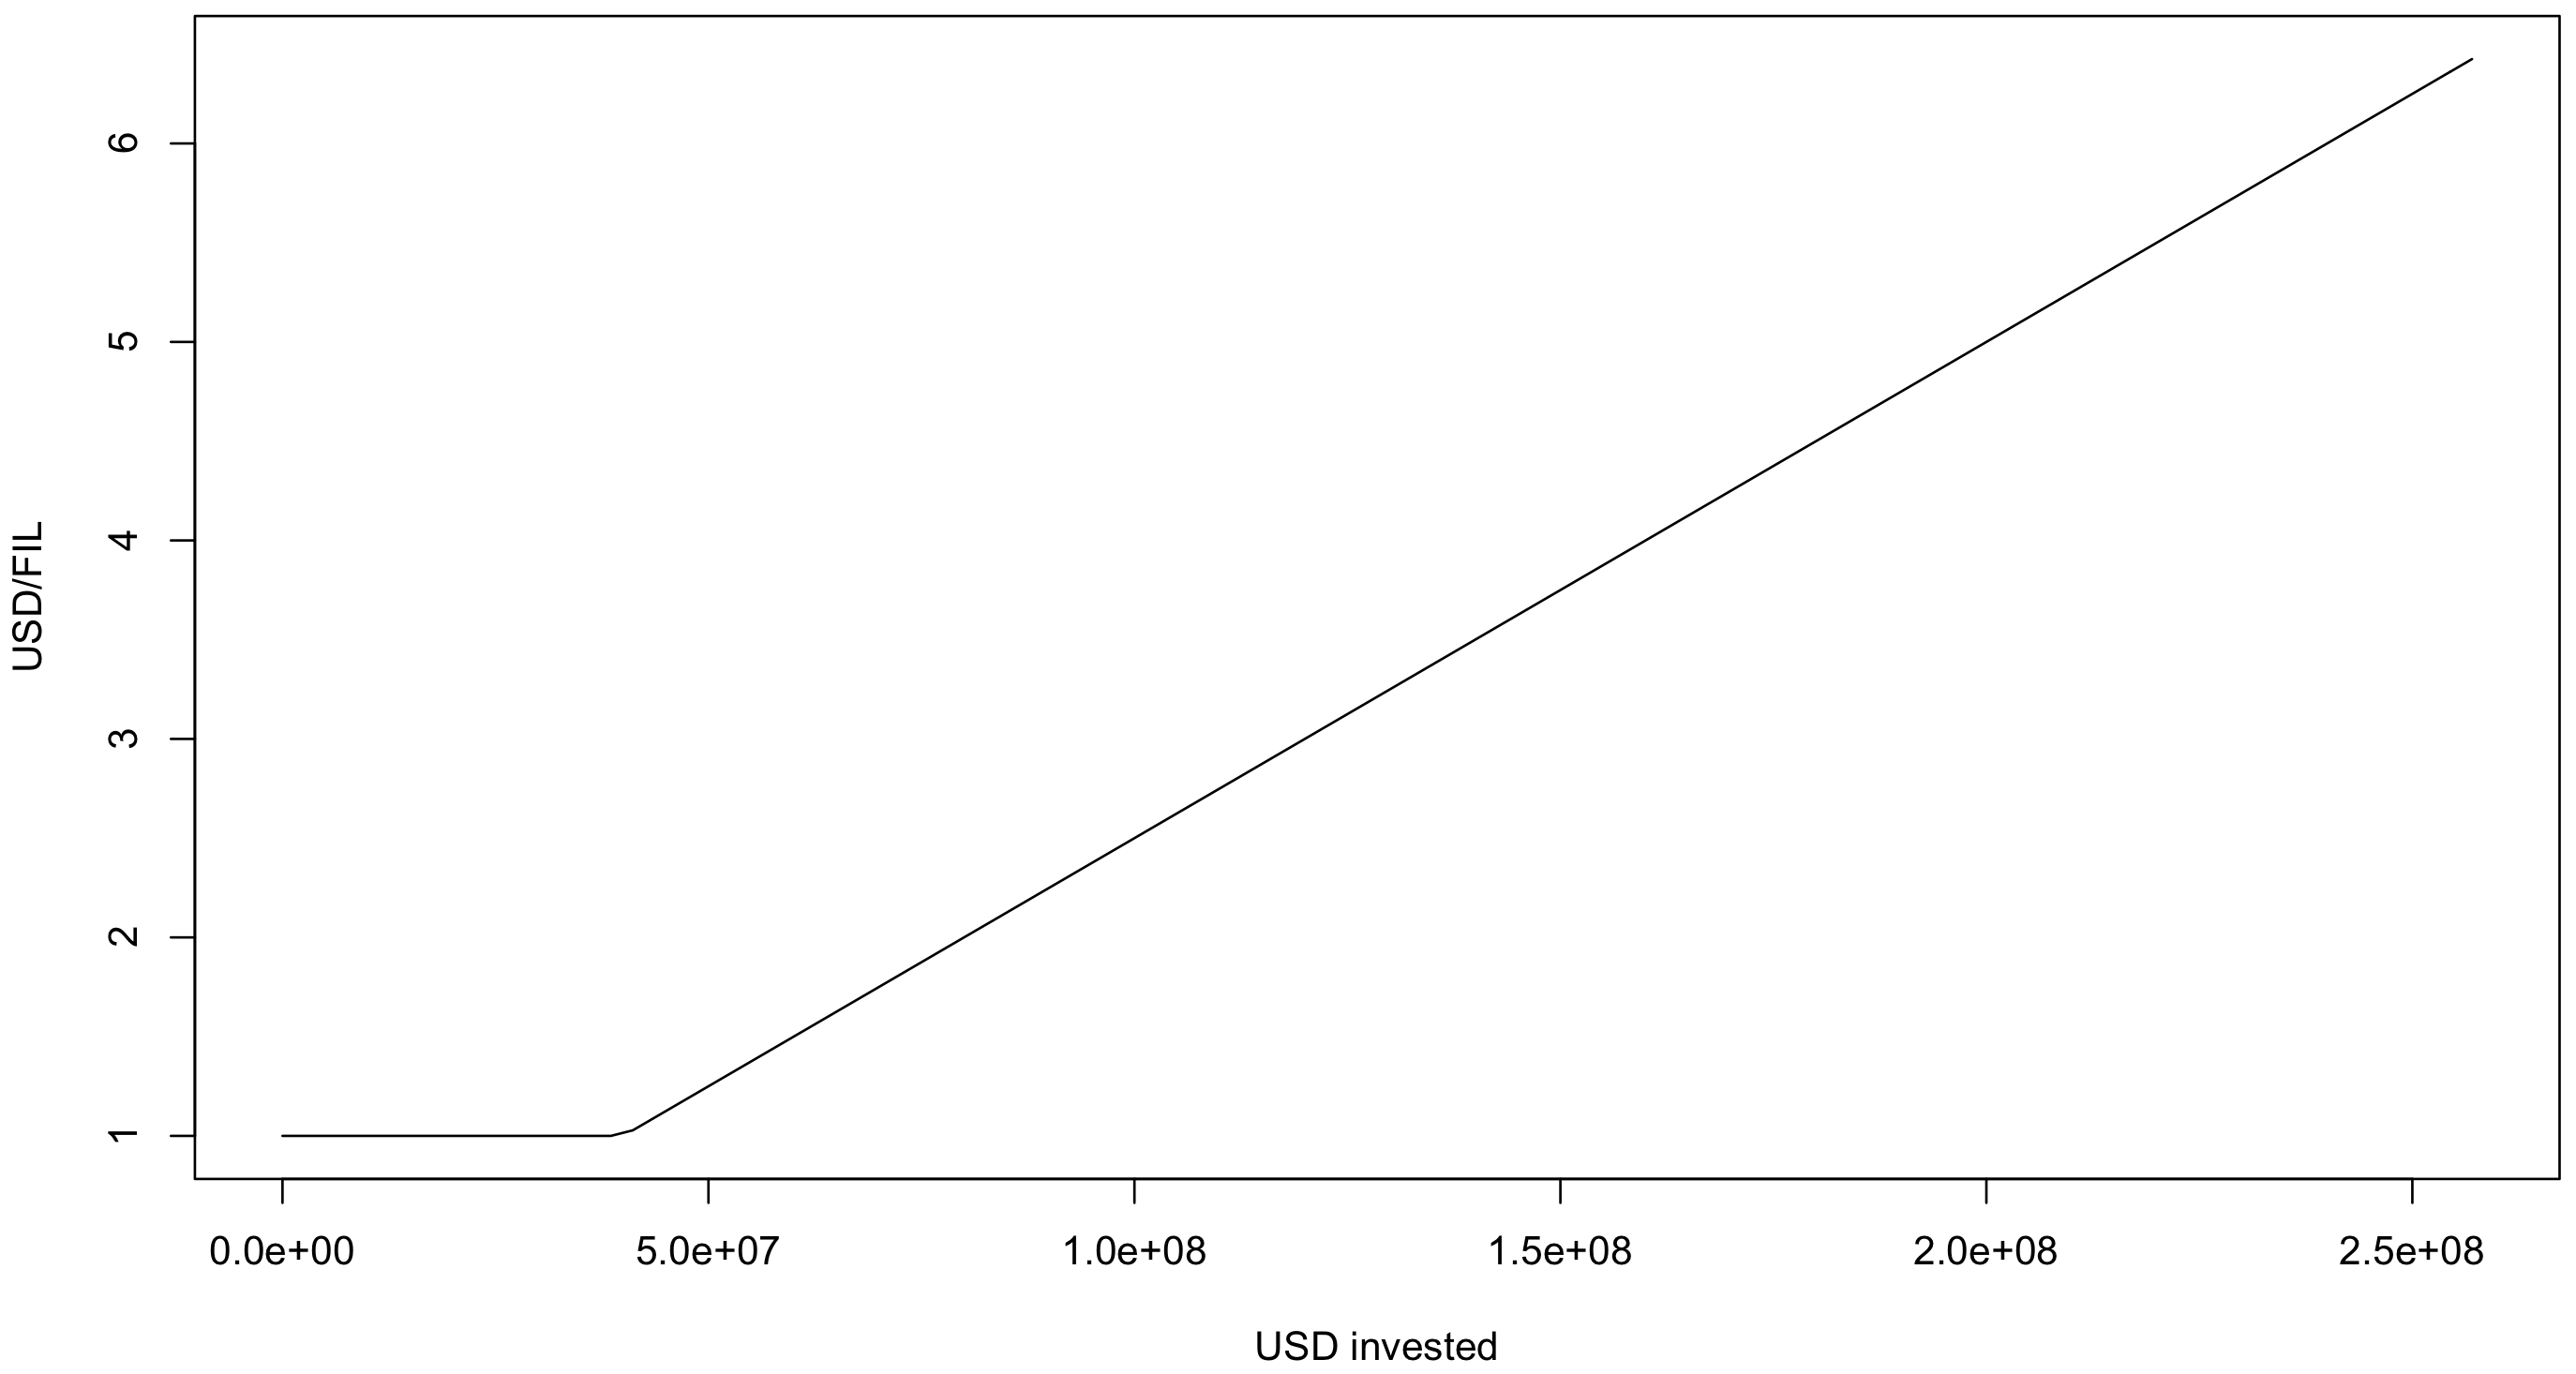
\includegraphics[width=0.4\textwidth]{filecoin-tokensale.png}
\caption{Filecoin sale price function}
\label{fig:sale-price}
\end{figure}
As a result, the closing price, past \$257'000'000 investments, can be estimated to be approximately \$6.425.
Hence, advisors and Protocol Labs Inc. itself were able to purchase for a price which is a factor of \$8.57 lower than the late investor.

\subsection{Questioning investors exclusion}



\section{Is the design technically feasible?}

In this section, technical details will be highlighted with reasoning whether the decisions stated in the Whitepaper\cite{filecoin} are chosen appropriately or arise potential weaknesses.
We further aim to make comparisons to more recent decentralized storage projects involving a blockchain, such as StorJ \cite{storj} and Sia \cite{Sia}.

\subsection{Proof-of-spacetime}

% use mindmap

\section{Is the design economically feasible?}

\section{Is this a pyramid scheme?}

\section{Is it a bubble?}

In a recent interview \cite{podcast}, Juan Benet compares Filecoin with Airbnb \cite{airbnb} where people can rent away storage, instead of their homes.
As of today (September 2017), Airbnb values at approximately \$31 billion while holding around 3 million listings in total \cite{airbnb-valuation}.
The average apartment in the United States was 934 square feet in 2016 \cite{housing-cnbc}.
In a hypothetical scenario, Airbnb is therefore valued \$$11.06$ per square feet. 
If one would compare this number to the median price per square feet in the United States, which is \$123 \cite{home-prices}, the Airbnb ecosystem diminishes the median price by a factor of $11.12$.
The average price for hard drives in 2017 is \$0.03 per Gigabyte \cite{hard-drive}.
Dividing the same factor as Airbnb applies for square feet to the storage price, the average Gigabyte in the Filecoin system results in \$0.0027.
This in fact means, the \$$257'000'000$ launched at the Filecoin ICO require $95'185'185'185$ Gigabyte ($95'185$ Petabyte) of storage to be offered by storage miners.
Considering that Dropbox \cite{dropbox} holds currently around $500$ Petabyte of user data \cite{dropbox-userdata}, one could argue that Filecoin is overvalued.


% Can use something like this to put references on a page
% by themselves when using endfloat and the captionsoff option.
\ifCLASSOPTIONcaptionsoff
  \newpage
\fi

% trigger a \newpage just before the given reference
% number - used to balance the columns on the last page
% adjust value as needed - may need to be readjusted if
% the document is modified later
%\IEEEtriggeratref{8}
% The "triggered" command can be changed if desired:
%\IEEEtriggercmd{\enlargethispage{-5in}}

% references section

% can use a bibliography generated by BibTeX as a .bbl file
% BibTeX documentation can be easily obtained at:
% http://www.ctan.org/tex-archive/biblio/bibtex/contrib/doc/
% The IEEEtran BibTeX style support page is at:
% http://www.michaelshell.org/tex/ieeetran/bibtex/
%\bibliographystyle{IEEEtran}
% argument is your BibTeX string definitions and bibliography database(s)
%\bibliography{IEEEabrv,../bib/paper}
%
% <OR> manually copy in the resultant .bbl file
% set second argument of \begin to the number of references
% (used to reserve space for the reference number labels box)
\begin{thebibliography}{1}

\bibitem{token-sale} "Filecoin Token Sale Economics", https://coinlist.co/static/media/Filecoin-Sale-Economics.0ae9a53f.pdf, accessed: September 25, 2017.

\bibitem{saft-agreement} "Simple Agreement for Future Tokens", https://coinlist.co/static/media/Protocol\%20Labs\%20-\%20SAFT\%20for\%20Filecoin\%20Token\%20Presale.6ddb6fb6.pdf, accessed September 25, 2017.

\bibitem{bubble} Blanchard, Olivier Jean. "Speculative bubbles, crashes and rational expectations." Economics letters 3.4 (1979): 387-389. %http://www.sciencedirect.com/science/article/pii/016517657990017X

\bibitem{pyramid-scheme} Gastwirth, Joseph L. "A probability model of a pyramid scheme." The American Statistician 31.2 (1977): 79-82.

\bibitem{angellist} "AngelList", https://angel.co/, accessed: September 22, 2017.

\bibitem{coinlist} "CoinList", https://coinlist.co/, accessed: September 22, 2017.

\bibitem{regulation-506} "Rule 506 of Regulation D", https://www.sec.gov/fast-answers/answers-rule506htm.html, accessed: September 22, 2017.

\bibitem{tribler} "Tribler Project", https://www.tribler.org/, accessed: September 22, 2017.

\bibitem{tribler-hurdles}
"Tribler Issue: blockchain-regulated markets", https://github.com/Tribler/tribler/issues/2559\#issuecomment-307353664, accessed: September 22, 2017.

\bibitem{storj} Wilkinson, Shawn, et al. "Storj a peer-to-peer cloud storage network." (2014).

\bibitem{filecoin} “FileCoin
whitepaper,” https://filecoin.io/filecoin.pdf, accessed: September 20, 2017.

\bibitem{filecoin-io} "FileCoin Website", https://filecoin.io/, accessed: September 20, 2017.

\bibitem{sia} Vorick, David, and Luke Champine. "Sia: Simple Decentralized Storage." (2014).

\bibitem{podcast} https://a16z.com/2017/09/14/networks-protocols-labs-tokens/

\bibitem{airbnb-valuation} https://expandedramblings.com/index.php/airbnb-statistics/

\bibitem{housing-cnbc} https://www.cnbc.com/2017/03/09/airbnb-closes-1-billion-round-31-billion-valuation-profitable.html

\bibitem{home-prices} http://www.realtytrac.com/news/home-prices-and-sales/march-q1-2016-home-sales-report/

\bibitem{hard-drive} https://www.backblaze.com/blog/hard-drive-cost-per-gigabyte/

\bibitem{dropbox-userdata} https://blogs.dropbox.com/tech/2016/03/magic-pocket-infrastructure/

\bibitem{airbnb} https://airbnb.com

\bibitem{dropbox} https://dropbox.com

\bibitem{consistent-hashing} Karger, David, et al. "Consistent hashing and random trees: Distributed caching protocols for relieving hot spots on the World Wide Web." Proceedings of the twenty-ninth annual ACM symposium on Theory of computing. ACM, 1997.

\bibitem{mojo-nation} Wilcox-O’Hearn, Bryce. "Experiences deploying a large-scale emergent network." Peer-to-Peer Systems (2002): 104-110.

\bibitem{peer-to-peer-xor} Maymounkov, Petar, and David Mazieres. "Kademlia: A peer-to-peer information system based on the xor metric." International Workshop on Peer-to-Peer Systems. Springer, Berlin, Heidelberg, 2002.

\end{thebibliography}

% biography section
% 
% If you have an EPS/PDF photo (graphicx package needed) extra braces are
% needed around the contents of the optional argument to biography to prevent
% the LaTeX parser from getting confused when it sees the complicated
% \includegraphics command within an optional argument. (You could create
% your own custom macro containing the \includegraphics command to make things
% simpler here.)
%\begin{biography}[{\includegraphics[width=1in,height=1.25in,clip,keepaspectratio]{mshell}}]{Michael Shell}
% or if you just want to reserve a space for a photo:


% You can push biographies down or up by placing
% a \vfill before or after them. The appropriate
% use of \vfill depends on what kind of text is
% on the last page and whether or not the columns
% are being equalized.

%\vfill

% Can be used to pull up biographies so that the bottom of the last one
% is flush with the other column.
%\enlargethispage{-5in}



% that's all folks
\end{document}


